\section{Par\'{a}metros de la Red}

\subsection{Alcance del documento}

El presente documento corresponde a una definici\'{o}n y descripci\'{o}n de las entradas y salidas del modelo de red a dise\'{n}ar. Para esto se ha definido una secci\'{o}n de an\'{a}lisis situacional donde se consideran aspectos del material con el que se dispone actualmente mediante el uso del sistema de control de tr\'{a}nsito del MOPT.

Dentro de este an\'{a}lisis se plantean las consideraciones realizadas y se brinda una explicaci\'{o}n general de la raz\'{o}n de ser de cada entrada y salida considerada. Dichos valores quedan a una revisi\'{o}n posterior donde como resultado se obtengan cambios que revelen dicha necesidad.

\subsection{Condiciones actuales}

El sistema del control de tr\'{a}nsito del MOPT cuenta con una serie de c\'{a}maras de vigilancia localizadas en diferentes puntos estrat\'{e}gicos dentro de la red abarcada, \'{e}stas se complementan con el uso de otro tipo de c\'{a}maras, las cuales sirven para llevar un registro o conteo de los veh\'{i}culos que pasen por determinada zona dentro de la intersecci\'{o}n. El funcionamiento de estos es simple, cada c\'{a}mara apunta a una determinada zona haciendo uso de una figura geom\'{e}trica seg\'{u}n sea configurada, en caso de que un veh\'{i}culo pase sobre esta zona bloqueando moment\'{a}neamente la visi\'{o}n de la c\'{a}mara, \'{e}sta lo contar\'{a} como un veh\'{i}culo m\'{a}s que pas\'{o} por ah\'{i}. De igual forma si el veh\'{i}culo queda posicionado sobre dicha zona, ser\'{a} contado al momento de abandonarla y que la c\'{a}mara pueda volver a ver la zona marcada originalmente.

Lo anterior se menciona, ya que fue considerado como una forma de captar el flujo de tr\'{a}fico que pasa por las intersecciones de la red de sem\'{a}foros. La idea es emplear estas c\'{a}maras como medio para captar la situaci\'{o}n del tr\'{a}fico de tal forma que al momento en que el sem\'{a}foro deje pasar veh\'{i}culos, la c\'{a}mara contar\'{a} la cantidad que dej\'{o} pasar durante un periodo determinado y luego brindar dicha informaci\'{o}n a la red de sem\'{a}foros de forma que estos puedan emplearla para tomar decisiones.

Una consideraci\'{o}n adicional es contar con una c\'{a}mara extra que apunte hacia la intersecci\'{o}n de las calles, debido a que en muchas ocasiones los conductores avanzan hacia \'{e}sta aun cuando saben que no les ser\'{a} posible pasar completamente y por causa de esto quedan bloqueando el paso de la intersecci\'{o}n afectando los conductores que viene de otros lados. Al contar con \'{e}sta c\'{a}mara extra se podr\'{i}a tomar como fuente la presencia o no de un veh\'{i}culo bloqueando el paso y de esta forma poder alterar el comportamiento de la red neuronal en los sem\'{a}foros para que se tome en cuenta este hecho y hacer lo posible por solventar el problema.


\subsection{Sobre autores previos}

Dado que se busca lograr una el manejo de una red de sem\'{a}foros, el modelo a ser planteado tiene que tomar en cuenta uno de los puntos principales mostrados en \cite{Srinivasan2006} %Srinivasan, Chee& Long (2006)
,en lo que respecta a formar un sistema de sem\'{a}foros basados en una red para el cual cada sem\'{a}foro corresponde a un nodo o “agente” como lo mencionan los autores. Resaltando parte del trabajo de los autores, se pretende que cada sem\'{a}foro pueda tener una noci\'{o}n de su entorno que puede ser considerada de la siguiente forma:

\begin{itemize}
	\item Conexiones directas: corresponde a los sem\'{a}foros que se encuentran directamente conectados con el agente en cuesti\'{o}n el n\'{u}mero de conexiones depender\'{a} de las v\'{i}as que hayan hacia otros sem\'{a}foros, es decir, si la calle o avenida de una direcci\'{o}n no cuenta con un sem\'{a}foro, \'{e}sta no ser\'{a} tomada en cuenta. Dadas las condiciones del \'{a}rea seleccionada, se podr\'{a} contar con un m\'{a}ximo de cuatro conexiones entre un nodo y sus contrapartes cercanas. 
	\item Rango de un \'{a}rea determinada: con este rango se pretende reducir la complejidad que conlleva estimar el estado de la red dado que se reduce el n\'{u}mero de sem\'{a}foros junto con los cuales cada nodo debe tomar en cuenta para llevar a cabo sus decisiones. Comprende un cantidad mayor de nodos que el caso anterior, con hasta tres calles de distancia entre cada nodo.
	
	\item Red completa: este caso implicar\'{i}a que cada nodo (sem\'{a}foro) dentro de la red tenga conocimiento de lo que pasa en esta ya sea que este afecte, sea afectado, o ninguna de las anteriores por parte de las decisiones tomadas por otros sem\'{a}foros.
	
	\item Conexiones directas extendidas: corresponde a una modalidad especial y la cual ser\'{a} utilizada dentro del programa de simulaci\'{o}n a emplear. Se hace uso de la idea b\'{a}sica de las conexiones directas pero cambiando el hecho de que si un sem\'{a}foro realiza un cambio, \'{e}ste avisar\'{a} a sus vecinos directos del mismo indicando la nueva informaci\'{o}n con la que est\'{a} trabajando de forma que se empiece un efecto en cadena de actualizaciones.

\end{itemize}


\subsection{Modelo de Funcionamiento}

La figura \ref{fig:light} muestra el modelo conceptual que se propone para el funcionamiento de cada sem\'{a}foro. Dentro de dicho gr\'{a}fico se debe destacar tres partes: modulador, NN y sistema principal

\begin{figure}[htp]
\centering
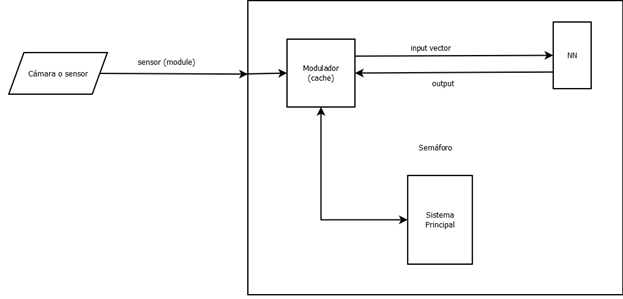
\includegraphics[scale=0.9]{images/light.png}
\caption{Diagrama de se\~{n}al de sem\'{a}foro}
\label{fig:light}
\end{figure}



\subsubsection{Modulador}

Corresponde a un proceso encargado de comunicar la red neuronal del sem\'{a}foro con las redes en otros sem\'{a}foros. En caso de funcionar con un sensor externo, recibir\'{a} los valores de este y mantendr\'{a} un cach\'{e} de la informaci\'{o}n solicitada a otro agentes vecinos. Los datos locales, junto con los datos de los vecinos ser\'{a}n formateados y enviados como entradas para la red neuronal (NN) la cual procesar\'{a} las entradas y generar\'{a} un resultado que ser\'{a} actualizado en el modulador.

La finalidad de \'{e}ste componente responde a la necesidad de contar con una fuente de informaci\'{o}n para los sem\'{a}foros vecinos la cual pueda ser utilizada para el procesamiento de la informaci\'{o}n, de esta forma si cualquier agente cercano solicita una actualizaci\'{o}n, el modulador responder\'{a} con los datos que posea en ese instante. Con funcionalidad anterior se logra mantener un proceso continuo y poco a poco se acerca a una convergencia adecuada de la red con respecto al estado de la misma.

Adicionalmente al proceso descrito anteriormente, se poseen adem\'{a}s de funcionalidades secundarias a modo de complemento como el caso de propagaci\'{o}n de informaci\'{o}n, solicitud de informaci\'{o}n y solicitud de actualizaci\'{o}n.

\begin{itemize}
	\item	Propagaci\'{o}n de informaci\'{o}n: representa la idea de difundir (broadcast) la informaci\'{o}n actualizada y mediante esto lograr actualizar a sem\'{a}foros vecinos lo antes posible.

	\item 	Solicitud de informaci\'{o}n: similar al caso anterior pero funcionando en periodos aleatorios de tiempo, seg\'{u}n sea requerido por el sem\'{a}foro para alguna situaci\'{o}n especial que se pueda presentar. Con esto se garantiza que aunque se tendr\'{a}n los datos m\'{a}s recientes sin importar si \'{e}stos fueron actualizados. Mediante este el modulador solicitar\'{a} informaci\'{o}n a sus vecinos y la almacenar\'{a} en el cach\'{e} correspondiente.

	\item	Solicitud de actualizaci\'{o}n: corresponde a un funcionamiento que pretende garantizar una sincronizaci\'{o}n de sem\'{a}foros en luz verde. Su finalidad es que si un sem\'{a}foro va a cambiar a luz verde, tratar de solicitar una actualizaci\'{o}n del estado de los sem\'{a}foros vecinos que puedan afectar el flujo actual.
\end{itemize}


Finalmente, es importante que el modulador ha sido concebido como un elemento independiente del sistema principal del sem\'{a}foro, dicha finalidad es garantizar una comunicaci\'{o}n continua de elementos mediante una estructura independiente. Por lo anterior, aunque el sem\'{a}foro est\'{e} ocupado ya sea si est\'{a} en mantenimiento o fuera de servicio, sus vecinos podr\'{a}n contar con la \'{u}ltima informaci\'{o}n si \'{e}sta se actualiza mediante sensores u otros elementos conectados a \'{e}ste.


\subsubsection{NN}
Representa a la red neuronal artifical (Neural Network) que ser\'{a} utilizada como el mecanismo para tomar decisiones seg\'{u}n la informaci\'{o}n proporcionada por el modulador. Una vez procesadas, se generar\'{a} una salida que volver\'{a} al modulador y se actualizar\'{a}. Al igual que el componente anterior, \'{e}ste tambi\'{e}n se concibe como un elemento separado \'{u}nicamente accesible por medio del modulador para lograr una encapsulaci\'{o}n e independencia del mecanismo para tomar decisiones que se pueda implementar, de \'{e}sta forma se puede actualizar o sustituir sin que se afecte el funcionamiento normal del sem\'{a}foro.


\subsubsection{Sistema Principal}

El sistema principal corresponde al n\'{u}cleo del sem\'{a}foro donde se llevan a cabo el manejo de los ciclos correspondientes y las actualizaciones de los tiempos par\'{a}metros que sean configurados al mismo. Para \'{e}ste modelo, el sistema contar\'{a} con dos modos de funcionamiento uno mediante ciclos y otro mediante decisiones. La modalidad mediante ciclos corresponde al funcionamiento por defecto con el que cuentan actualmente los sem\'{a}foros al tener pre establecidos diferentes tiempos para las luces de cada estado. Por su parte la modalidad por decisiones corresponde al uso del modulador y las redes neuronales, los cuales indicar\'{a}n al sem\'{a}foro c\'{o}mo actuar en un tiempo determinado. 

Para el proceso de simulaciones, se contar\'{a} con ambas modalidades de forma que se pueda realizar pruebas independientes en caso de que se requieran comparar resultados. Adicionalmente, se ha considerado ponerlas a operar simult\'{a}neamente con el fin de tener un modo de respaldo en caso de que el otro falle, en otras palabras se contar\'{a} con la modalidad por decisiones como el principal y el modo por ciclos como secundario, en caso de que el primero falle el siguiente entrar\'{a} en funcionamiento.

Adicionalmente, al modelo anterior se suman algunos niveles de interacci\'{o}n, los cuales deben ser considerados para los diferentes par\'{a}metros de entrada y salida en cada procesamiento. Se poseen dos niveles: entre nodos o agentes y entre la red neuronal y el agente.

\subsection{Interacci\'{o}n entre nodos}

Como bien se ha mencionado anteriormente, el modelo que se busca probar consiste de una red de sem\'{a}foros dentro del \'{a}rea definida la cual pueda funcionar en forma conjunta y donde cada sem\'{a}foro (agente o nodo) pueda tomar decisiones basados en el entorno que los rodea. Por lo tanto algunos de los par\'{a}metros que han de ser recibidos por las redes neuronales en cada uno de \'{e}stos, provendr\'{a}n de otros nodos es decir, de una fuente externa (E).

\subsection{Interacci\'{o}n entre la red neuronal y el agente}

Caso contrario al anterior, gran parte de los par\'{a}metros que recibir\'{a} la red neuronal ser\'{a}n proporcionados por el agente donde se encuentra la red. Esto se debe al hecho de que los datos necesarios para tomar decisiones corresponder\'{a}n al conocimiento adquirido por el sem\'{a}foro ya se por configuraci\'{o}n previa o como parte de indicaciones parametrizadas que se env\'{i}en al mismo por alg\'{u}n medio. Sin importar el caso, se requiere que estos datos se encuentren presentes en el sem\'{a}foro ya que se han considerado como importantes al momento de realizar la toma a decisiones por parte de la red. A estos se le considera como una fuente interna o local (L).

De esta forma, para cada entrada y salida se especifica si la misma proviene o ser\'{a} utilizada dentro o fuera del agente. Definido lo anterior, la siguiente secci\'{o}n presenta las entradas consideradas para llevar a cabo el dise\'{n}o del modelo.

\subsection{Entradas de la Red}

Considerando las condiciones actuales, y algunos de los conocimientos brindados por autores como \cite{Srinivasan2006} y \cite{Gilmore1993} %Srinivasan, Chee \& Long (2006) y Gilmore, J. F., y Elibiary, K. J. (1993), 
se consideraron como par\'{a}metros de entrada los siguientes puntos:

\begin{enumerate}
	\item \textbf{Capacidad de carga de la calle que conduce al sem\'{a}foro:} tomando como idea el punto planteado por Gilmore, J. F., y Elibiary, K. J. (1993), una de las entradas corresponder\'{a} a la capacidad de carga que posea dicha calle, esto con el fin de determinar si la calle est\'{a} llegando a su l\'{i}mite y se requiere realizar ajustes extraordinarios que permitan “despejar” los veh\'{i}culos de forma r\'{a}pida para evitar el desarrollo de una congesti\'{o}n. Se har\'{a} una variante que corresponde a dividir la calle en cada carril tomando en cuenta que la capacidad m\'{a}xima estimada para un  carril est\'{a} dentro del rango de 600 a 700 carros por hora (cuando se cuenta con sem\'{a}foro). De \'{e}sta forma la red podr\'{a} determinar cuando el total de la calle o por carril se encuentra saturado o est\'{a} llegando a puntos que provoquen esto. Como parte del c\'{a}lculo se tomar\'{a} la Relaci\'{o}n volumen / capacidad que si es m\'{a}s de 0.8 la calle est\'{a} saturada

	\item \textbf{Cantidad esperada de veh\'{i}culos que deber\'{i}a llegar:} este corresponde a la estimaci\'{o}n realizada por el sem\'{a}foro ubicado directamente en la intersecci\'{o}n a esta. Con esto se busca determinar si de acuerdo a estados anteriores, la calle est\'{a} llegando al l\'{i}mite de su capacidad

	\item \textbf{Cantidad real de veh\'{i}culos que est\'{a}n llegando a este sem\'{a}foro:} como su nombre lo indica, se diferencia a la anterior a que este puede ser un n\'{u}mero diferente al estimado, lo cual reflejar\'{i}a un atraso causado por un evento ocurrido en el sem\'{a}foro anterior. Con esto se busca determinar la presencia de alg\'{u}n factor que afecte el flujo normal de los autom\'{o}viles. Cabe mencionar que para garantizar un control del \'{a}rea, se deber\'{a} contar con un dato proveniente por cada nodo conectado, es decir cuando se est\'{e} moviendo los carros de las avenidas el dato corresponder\'{a} a las avenidas conectadas y de forma similar para las calles.

	\item \textbf{Presencia de paradas de buses, taxis o zonas de carga y descarga:} Corresponde a paradas fijas las cuales permanecen ocupadas en todo momento para el fin establecido de forma que la calle ve reducida su capacidad para albergar veh\'{i}culos.

	\item \textbf{Velocidad m\'{a}xima permitida para el carril o la calle correspondiente:} Esto permitir\'{a} a la red estimar el tiempo que tardar\'{a}n determinados veh\'{i}culos en atravesar la intersecci\'{o}n.

	\item \textbf{Presencia de carriles con giros (dos direcciones):} Dado que no todos los carriles siguen una direcci\'{o}n, el nodo debe estar consciente de que uno o m\'{a}s carriles pueden permitir a los veh\'{i}culos tomar otra ruta por lo que \'{e}ste movimiento puede afectar dependiendo de la situaci\'{o}n en la que se encuentre la zona hacia la que ha de girar el veh\'{i}culo.

	\item \textbf{Cantidad de carriles con m\'{a}s de una direcci\'{o}n:} corresponden a los carriles en los cuales los veh\'{i}culos pueden continuar directo, o doblar tomando alguna direcci\'{o}n permitida por la demarcaci\'{o}n establecida para esa calle. De esta forma la red tendr\'{a} en cuenta que determinado n\'{u}mero de veh\'{i}culos pueden tomar rutas alternativas dirigidas a otros nodos con los que mantienen comunicaci\'{o}n.

	\item \textbf{Delay sugerido para cambiar a luz verde:} tiempo en segundos que recomienda esperar el nodo vecino para realizar el cambio a luz verde, de forma que se optimice el uso de la luz verde.
\end{enumerate}


El cuadro \ref{tab:nninputs} resume los datos mencionados y se especifica la fuente (externa o local) de los mismos .

\begin{table}[H]
	\centering
	\begin{tabular}{p{8.5cm}|c}
		\multicolumn{1}{c}{\centering\textbf{Par\'{a}metro}} & \multicolumn{1}{c}{\centering\textbf{Fuente}}\\
		\hline
		\hline
		Capacidad de carga de la calle que conduce al sem\'{a}foro & Local\\
		Cantidad esperada de veh\'{i}culos a llegar & Externa\\
		Cantidad real de veh\'{i}culos recibidos & Externa\\
		Presencia de paradas de autobuses, taxis o zonas de carga y descarga & Local\\
		Velocidad m\'{a}xima permitida para el carril o la calle correspondiente & Local\\
		Presencia de carriles con giros & Local\\
		Cantidad de carriles con m\'{a}s de una direcci\'{o}n & 72\\
		Delay sugerido para cambiar a luz verde & Externo / local\\
		\hline
	\end{tabular}
	\caption{Resumen entradas de red}
	\label{tab:nninputs}
\end{table}


\subsection{Salidas de la red}

Tomando como base las entradas anteriores, se han definido las siguientes salidas para la red neuronal en cada sem\'{a}foro o nodo del sistema.

\begin{enumerate}
	\item	\textbf{Duraci\'{o}n en segundos de la luz verde} sumada con el verde intermitente para indicar que el sem\'{a}foro est\'{a} a punto de realizar el cambio a luz roja. Para este caso la luz \'{a}mbar se suma a la verde, dado que es com\'{u}n el hecho de ver personas pasar aun cuando ven esta luz por lo que el sem\'{a}foro se considera con dos estados nada m\'{a}s verde y rojo

	\item \textbf{Umbral m\'{a}ximo de espera entre el \'{u}ltimo veh\'{i}culo que pas\'{o} y el siguiente:} es decir cu\'{a}nto tiempo tiene que esperar el sem\'{a}foro despu\'{e}s de haber pasado el \'{u}ltimo veh\'{i}culo para no cambiar a luz roja por la falta de demanda en el mismo.

	\item \textbf{Delay sugerido para cambiar a luz verde:} con esta salida se busca una mayor prolongaci\'{o}n de las luces verdes en las direcciones que se necesitan. De esta forma si en una calle hay pocos o ning\'{u}n carro esperando al cambio de luz entonces prolongar la duraci\'{o}n de la luz verde en el otro sentido (donde s\'{i} se encuentran veh\'{i}culos utiliz\'{a}ndola), por lo anterior la luz roja del siguiente nodo (sem\'{a}foro) cambiar\'{i}a hasta que suficientes carros se encuentren cerca o a punto de llegar a \'{e}ste.
 
\end{enumerate}

La tabla \ref{tab:nnoutputs} muestra un resumen de los datos considerados como salidas.

\begin{table}[H]
	\centering
	\begin{tabular}{p{8.5cm}|c}
		\multicolumn{1}{c}{\centering\textbf{Par\'{a}metro}} & \multicolumn{1}{c}{\centering\textbf{Fuente}}\\
		\hline
		\hline
		Duraci\'{o}n en segundos de la luz verde m\'{a}s duraci\'{o}n en segundos de la luz ambar(planes de luces del sem\'{a}foro) & Local y externo\\
		Umbral de espera & Local\\
		Delay sugerido para cambiar a luz verde & Externo\\
		\hline
	\end{tabular}
	\caption{Resumen salidas de red}
	\label{tab:nnoutputs}
\end{table}

\subsection{Salidas del modulador}
Con la red neuronal se busca obtener salidas m\'{a}s sencillas que no requieran c\'{a}lculos adicionales por lo tanto se ha considerado delegar la generaci\'{o}n de ciertas salidas al modulador el cual ha de tomar algunos de los datos que maneja para la red junto con las salidas de la misma con el fin de obtener el valor buscado. Cabe mencionar que estos datos no se ver\'{a}n afectados por los c\'{a}lculos que realice el modulador y que dichos resultados simplemente corresponden a los datos que manipule la red.

\begin{enumerate}
	\item \textbf{Cantidad estimada de veh\'{i}culos que han de pasar:} Dependiendo de duraci\'{o}n de la luz verde se estimar\'{a} una cantidad de veh\'{i}culos que pasaran por el sem\'{a}foro permitiendo indicarle al siguiente sem\'{a}foro la cantidad estimada de veh\'{i}culos que van a llegar.

	\item \textbf{Relaci\'{o}n volumen / capacidad} que si es m\'{a}s de 0.8 la calle est\'{a} saturada para la red tomando en cuenta los datos del tiempo anterior y de esta forma saber si se requiere dejar activas por mas tiempos las luces verdes. Corresponde a un funcionamiento b\'{a}sico, si el nodo vecino presentaba m\'{a}s carga, el nodo actual ayudar\'{a} brindando m\'{a}s soporte.
	
\end{enumerate}